% Introduction to the section
%
This section focuses on a detailed overview of each component required to build and train the Machine Learning model.
It will go through each type of model used in this investigation and breaks them part by part to overview potential strengths and weaknesses.
In addition, every optimiser will be discussed in the growing complexity to visualise their development process over time and pick the most processing for the final goal.
% Classical RNN consists primarily of three layers, represented in \mbox{Figure~\ref{fig:RNN-structure}}.
\begin{figure}[htbp]
    \centering
    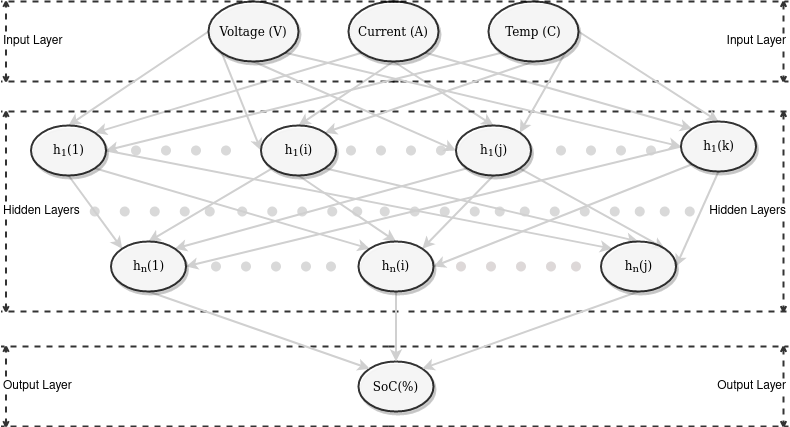
\includegraphics[width=\columnwidth]{II_Body/images/SoC-RNN.png}
    \caption{Universal structure of RNN for SoC estimation.\textcolor{red}{Ready, but not eager to eradicate it.}}
    \label{fig:RNN-structure}
\end{figure}

%  Model Structure
% Parameters definition layers and neurons selection
%
\subsection{Model structure and implementation} \label{subsec:structure}
The general summary model structure is represented in \mbox{Figure~\ref{fig:RNN-structure}}, with three feature inputs and a single output.
The most efficient number of layers and hidden neurons for the State of Charge estimation application was determined to be 3, with 43 per each.
Since the output consists of only a single sample, it is defined by a fully connected layer - a dense layer with a single neuron.
That makes a total of 130 cells for each implemented case.
% In case the article did not specify the number of neurons per layer, the following equations have been used to get the initial raw estimation~\cite{eckhardt_choosing_2018}:
% \begin{equation}
%     \begin{split}
%         N_h &= \frac{N_s}{ a \left(N_i+N_o \right)} \ \ OR \ \ N_h = \frac{2}{3}\left(N_i+N_o \right) \\
%         N_i &\rightarrow \text{Number of input neurons} \\
%         N_o &\rightarrow \text{Number of output neurons} \\
%         N_s &\rightarrow \text{Number of samples in training data set} \\
%         \alpha &\rightarrow \text{An arbitrary scaling factor 2(5)-10}
%     \end{split}
% \end{equation}
%**Contrary to Hidden Layers as per their name, they obey only internally defined logic and connections.
%**That is why models are stable and reliable once created, cannot be changed, only retrainable with different data.
%A standard Hidden layer consisting of fully connected neurons called a Dense Layer.
%A standard Hidden layer, consisting of fully connected neurons and only one or no activation function, is called a Dense Layer.
%Within each cell of a Dense layer lies a single activation function.

%An Output Layer gets created from Dense Layer and commonly with no Activation function.
%: \textit{Simple, Exponential or Rectified Linear; Sigmoid and Hyperbolic Tangent functions}. \\
% \begin{itemize}
%     \item \textit{linear} - Simple Linear function
%     \item \textit{elu} - Exponential Linear function
%     \item \textit{relu} - Rectified Linear unit function
%     \item \textit{sigmoind} - Sigmoid function $sigmoid(x) = 1/1(1+exp(-x)$
%     \item \textit{tanh} - Hyperbolic Tangent function $$
% \end{itemize}

% Tanh and sigmoid definitions, equations and dropout.
%
Several activation functions for those layers are widely used in machine learning libraries for time series problems~\cite{amidi_cs_2018}.
For the SoC prediction problem, all authors used the same function.
Experimentally confirmed that the best one for all hidden layers is the hyperbolic \textit{tangent} function, \mbox{Equation~\ref{eq:tanh}}.
The output layer uses a \textit{sigmoid} function as an activation to bound the result between zero and one, indicating the percentage of the charge \mbox{Euation~\ref{eq:sigmoid}}.
A dropout layer technique with a 20\% cut-off has been applied to all hidden layers to prevent early data overfitting over long training periods.
\begin{equation}
    tanh(x) = \frac{sinh(x)}{cosh(x)}=\frac{e^x-e^{-x}}{e^x+e^{-x}}
    \label{eq:tanh}
\end{equation}
\begin{equation}
    \sigma(x) = \frac{1}{1+e^{-x}}
    \label{eq:sigmoid}
\end{equation}
%
%
%The common usage of the Dense layer in this paper is the Output Layer with no activation functions and a single neuron representing a single output SoC value.
%To apply multiple different without overcomplicating neurons, multiple layers with different or the same number of neurons or activations functions are applied.
%The more Hidden layers a network contains - the deeper and computationally complex a network becomes, also referred to as Deep Neural Networks. 
% Choosing the number of neurons for a first Hidden Layer does not have a golden rule.
% For this article, the following formula helps to make a good initial estimate based on the number of samples, Input and Output.\\
% \textbf{Equation}\\
% A common practice is to narrow each following Neurons by two from the previous one, to make a more accurate capture.
% To avoid overfitting data, except for data normalisation and Input sample shuffling in stateless models, a Dropout technique gets applied.
% Tensorflow has an internal implementation of Dropout for GRU and LSTM layers. A value of 0.2 (20\%) was applied to all RNN layers to minimise the overfitting possibility.

% Intro to vanishing gradient problem and gentle move to LSTM and GRU.
% Requires editing below
The efficiency of an RNN over time series problem is defined by the ability of the neurons to store memory as an internal state.
With time, the memory of long passed samples may fade away.
The problem is called vanishing gradient when the value to update network weights shrinks as it propagates through time~\cite{rasifaghihi_predictive_2020}.
Long-term dependencies are not captured since layers with a slight gradient do not significantly affect the system due to insufficient weight change~\cite{rasifaghihi_predictive_2020,hochreiter_vanishing_1998}.
The more complicated structures of neurons tend to solve that problem.
% The gradient is the value used to update Neural Networks’ weight.
%"Therefore, layers that get a small gradient do not learn, and they cause the network to have short-term memory."
% https://www.bioinf.jku.at/publications/older/2304.pdf
%"With gradient-based learning methods, the current error signals have to 'flow back in time over the feedback connections to past inputs for building up adequate input storage. Long-term dependencies are hard to learn because of insufficient weight changes."

% Introduction statement to Gated Recurrent Unit and Long-Short Term Memory.
%
Two commonly used Recurrent Neural Network utilises memory cells: Gated Recurrent Unit (GRU) and Long Short-Term Memory (LSTM), with possible extensions implemented by the articles' authors.
% The GRU implementation will be used as a stateful technique by preserving a state from batch to batch with a single sample at a time.
The GRU and LSTM will take a stateless approach, providing a fixed number of timestamps for all implemented models.
The stateless implementations and non-gradient calculus-based optimisation algorithms will not be used as part of the research as their effectiveness has not been proven during preliminary work for this case.
%Implementation of the model based on simple RNN using multi-layer Dense(X) networks.~\cite{lees2010theoretical}
% a basic version of Recurrent Neural Network consists of fundamental layers with some neurons.
% \subsubsection{Implementation}
%     The input data for a network has been created using the Windowing technique, where \textbf{216k} sample of battery data, consisting of State Of Charge only, were separated on 500 sample windows.
%     As a result, the model outputs a single sample as SoC at the next Time Step. Using the Tensorflow library and calculating the number of Neurons using recommended formula \\
%     \textbf{THIS IS THE BEST PLACE FOR IT}. No other place suites as much.
%     The structure of the model ha\subsection{Training and Validation}

%s the following form. (Few Dense Layers+Dropount).
%     A Dropout layer has been used to prevent data overfitting. The selection of activation functions has been made through the data properties, which model has to fit in multiple trials.
% \subsubsection{Observation}
%     A simple Recurrent Neural Network has proven effective with simple Linear problems. However, with the battery state of charge, it cannot capture complicated features like the transition between Discharge and Charge or the process of Constant-Voltage Constant-Current charging. In applying battery utilisation inside Electrical Vehicle, this approach can be used only with some additional logic, such as Kalman Filters.
%     The best approach is to introduce more information about battery state and use a more complicated version of Time Series capable of memorising features with time, such as LSTM~\ref{sec: LSTM} and GRU~\ref{sec: GRU}.
    % The prediction results are discussed in Section~\ref{sec:results}.
%\subsection{Stateful Gradient Recurrent Unit (GRU) Algorithms and Implementations} \label{subsec:GRU}
%\subsection{LSTM with Attention}\label{sec:lstm-attention}
LSTM and GRU models made the most comonly used implemtation of Time -series predictions. TadeleMamo2020 research was intended to determine waknesses and improve the model introducing addition techniques into the default structure of training model***. \\
THe attention mechanissm used in ... \\
THe intention was to capture ... \\
\subsection{Implementation}
    Attention layer implementation was taken from \textbf{refernece} github repositry of ....
    
Implementation of the model based on TadeleMamo 2020 as the most recent and how to implement improvement to the model to make it better. Gracefully transition idea from here to my model, it is similar.
